\documentclass{article}
\usepackage{amsmath}
\usepackage{amsfonts}
\usepackage{amssymb}
\usepackage{multicol}
\usepackage{graphicx}

\graphicspath{ {./images/} }

\setlength{\parindent}{0pt}

\begin{document}

\section*{04/01/2024}
\subsection*{PHYS31.01: Analytical Physics I - Lecture}
        \begin{enumerate}
            \item \textbf{Momentum}
             - product of mass and velocity. A vector quantity expressed as:
            \begin{align*}
                \vec{p}&=m\vec{v} 
            \end{align*}
            \item \textbf{Impulse}
            - difference between the final and the initial momenta of the object.
            \begin{align*}
                \vec{J}&=\vec{p}_{f}-\vec{p}_{i}=\Delta\vec{p} 
            \end{align*}
            \item \textbf{Derivative of Momentum}
            - by getting the time derivative of momentum, then we have:
            \begin{align*}
                \frac{d\vec{p}}{dt}&=m\frac{d\vec{v}}{dt}=m\vec{a} \\
                \Rightarrow\frac{d\vec{p}}{dt}&=\vec{F}_{net}=m\vec{a}
            \end{align*}
            \item \textbf{Force Applied by Collision}
            - the force applied by an object to another colliding object is then determined by:
            \begin{align*}
                \vec{F}&=\frac{d\vec{p}}{dt}
            \end{align*}
            \item \textbf{Average Collission Force}
            - the average force on the moving object is:
            \begin{align*}
                \vec{F}_{ave}&=\frac{\Delta\vec{p}}{\Delta t} \\
            \end{align*}    
            where $\Delta t$ is the \textbf{contact time}.
            \item \textbf{Momentum Conservation Principle}
            - In the absence of net external force, the total momentum of the system is conserved.
            \begin{align*}
                \sum \vec{F}_{ext}&=0 \\
                \vec{p}_{sys}&=constant \\
                \vec{F}_{net}&=\frac{d\vec{p}}{dt}=0
            \end{align*}  
            \begin{enumerate}
                \item Example 1: \\
                \begin{center}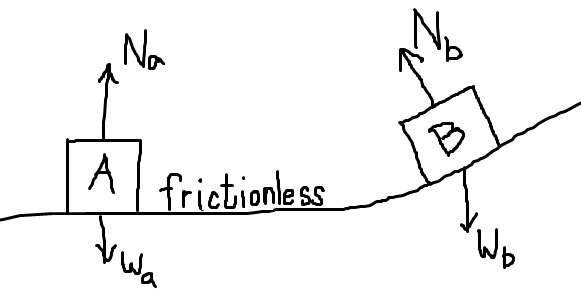
\includegraphics[width=10cm, height=5cm]{1.PNG}\end{center}
                \begin{align*}
                    \vec{F}_{ext. net}&=\vec{W}_a+\vec{W}_b+\vec{N}_a+\vec{N}_B
                \end{align*}  
                The total momentum of the system of the two blocks is \textbf{NOT conserved}. \\
                \item Example 2: \\
                \begin{center}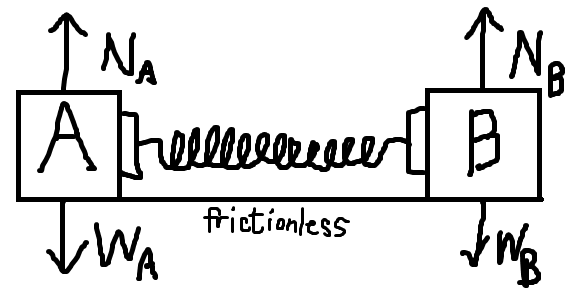
\includegraphics[width=7.5cm, height=3.75cm]{2.PNG}\end{center}
                \begin{align*}
                    \vec{F}_{ext. net}&=0
                \end{align*} 
                Momentum conservation principle \textbf{HOLDS}. \\
                \item Example 3: \\
                Consider the two cars that will meet at the intersection box as shown below: \\
                \begin{center}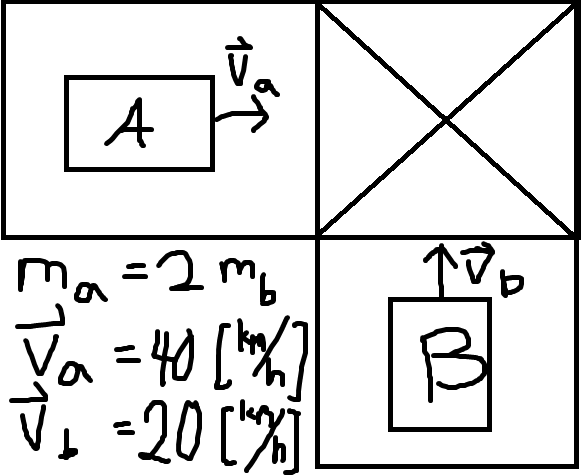
\includegraphics[width=5cm, height=5cm]{3.PNG}\end{center}
                What will be the velocity of the cars if they stick together after their collision?
                \begin{align*}
                    \vec{p}_{i sys}&=\vec{p}_{iA}+\vec{p}_{iB} \\
                    &=m_av_a+m_bv_b \\
                    &=(2m_b)(40[frac{km}{h}]\hat{i})+(m_b)(20[\frac{km}{h}]\hat{j}) \\
                    &=m_b(80[\frac{km}{h}]\hat{i}+20[\frac{km}{h}]\hat{j})
                \end{align*} 
                \begin{align*}
                    \vec{p}_{f sys}&=(m_a+m_b)\vec{v}_f \\
                    &=3m_b\vec{v}_f
                \end{align*} 
                \begin{align*}
                    \vec{p}_{i sys}&=\vec{p}_{f sys} \\
                    m_b(80[\frac{km}{h}]\hat{i}+20[\frac{km}{h}]\hat{j})&=3m_b\vec{v}_f \\
                    \vec{v}_f&=\frac{1}{3}(80[\frac{km}{h}]\hat{i}+20[\frac{km}{h}]\hat{j})
                \end{align*} 
            \end{enumerate}
            \item \textbf{Elastic and Inelastic Collision}
            \begin{enumerate}
                \item Elastic Collision - momentum of the system \textbf{IS} conserved, but kinetic energy \textbf{IS} conserved.
                \item Inelastic Collision - momentum of the system \textbf{IS} conserved, but kinetic energy is \textbf{NOT} conserved.
            \end{enumerate}
            \item \textbf{Elastic Collision in 1-D}
            \begin{center}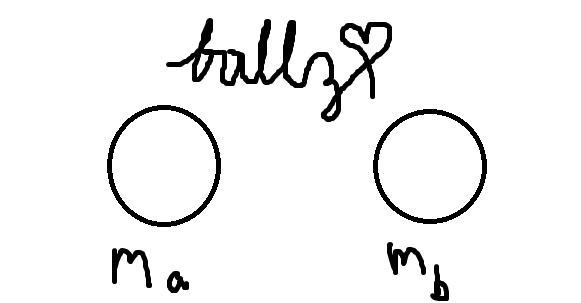
\includegraphics[width=5cm, height=2.5cm]{4.PNG}\end{center}
            Momentum:
            \begin{align*}
                m_av_{a_i}+m_bv_{b_i}&=m_av_{a_f}+m_bv_{b_f} \\
                m_a(v_{a_i}-v_{a_f})&=m_b(v_{b_f}-v_{b_i}) \\
            \end{align*}
            Kinetic Energy:
            \begin{align*}
                \frac{1}{2}m_av_{a_i}^2 + \frac{1}{2}m_bv_{b_i}^2&=\frac{1}{2}m_av_{a_f}^2 + \frac{1}{2}m_bv_{b_f}^2 \\
                m_a(v_{a_i}^2-v_{a_f}^2)&=m_b(v_{b_f}^2-v_{b_i}^2) \\
            \end{align*}
            \begin{align*}
                \Rightarrow v_{a_i}+v_{a_f}&=v_{b_f}+v_{b_i} \\
                \Rightarrow v_{a_i}-v_{b_i}&=-v_{a_f}+v_{b_f}
            \end{align*}
            \begin{enumerate}
                \item Example 1: \\
                Assuming elastic collision. What are the values of $v_af$ and $v_bf$?
                \begin{align*}
                    \vec{P}_{i sys}&=\vec{P}_{ia}+\vec{P}_{ib} \\
                    &=m_av_{a_i}+m_bv_{b_i} \\
                    &=16[kg\frac{m}{s}]\hat{i} \\
                \end{align*}  
                \begin{align*}
                    \vec{P}_{f sys}&=m_av_{a_f}+m_bv_{b_f} \\
                    (2 kg)(v_{a_f})+(3 kg)(v_{b_f})&=16[kg\frac{m}{s}]\hat{i} \\
                \end{align*}
                \begin{align*}
                    v_{b_f}-v_{a_f}&=3[\frac{m}{s}]\hat{i} \\
                    v_{b_f}&=3[\frac{m}{s}]\hat{i} + v_{a_f} \\
                    2v_{a_f} + 3v_{b_f}&=16 \\
                    2v_{a_f} + 3(3+v_{a_f})&=16 \\
                    5v_{a_f}&=7 \\
                    v_{a_f}&=1.4[\frac{m}{s}]\hat{i} \\
                    v_{b_f}&=4.4[\frac{m}{s}]\hat{i} \\\\\\
                \end{align*}
            \end{enumerate}
        \end{enumerate}
\subsection*{M31.2: Mathematical Analysis IB}
    \begin{enumerate}
        \item \textbf{Integration of Partial Fraction Decomposition:} \\
        \begin{enumerate}
            \item LOL 1
            \begin{align*}
                \int \frac{1}{x^2-x} \,dx \\
                \frac {1}{x(x-1)}&=\frac{A}{x}+\frac{B}{x-1} \\
                1&=A(x-1)+B(x) \\
                1&=A+B(x)-(A) \\
                \Rightarrow A&=-1 \\
                \Rightarrow B&=1 \\
                &=\int [\frac{-1}{x}+frac{1}{x-1}] \,dx \\
                &= -\int \frac{1}{x} \,dx + \int \frac{1}{x-1} \,dx \\
                &= -ln|x|+ln|x-1| \\
                &= ln|\frac{x-1}{x}|
            \end{align*}
            \item LOL 2
            \begin{align*}
                \int \frac{x+3}{(x-1)(2x+1)} \,dx \\
                \frac {x+3}{(x-1)(2x+1)}&=\frac{A}{(x-1)}+\frac{B}{(2x+1)} \\
                x+3&=A(2x+1)+B(x-1) \\
                \textit{Let $x=1$}&\Rightarrow 4=3A \\
                \textit{Let $x=-\frac{1}{2}$}&\Rightarrow \frac{5}{2}=-\frac{3}{2}B \\
                A=\frac{4}{3}&,B=-\frac{5}{3}\\
                &=\frac{4}{3}\int\frac{1}{x-1}\,dx - \frac{5}{3}\int\frac{1}{2x+1}\,dx \\
                &=[(\frac{4}{3})ln|x-1|]-[(\frac{5}{3})(\frac{1}{2})ln|2x+1|]+C
            \end{align*}
            \item LOL 3
            \begin{align*}
                \int \frac{x+1}{(x)(x^2+1)} \,dx \\
                \frac {x+1}{(x)(x^2+1)}&=\frac{A}{(x)}+\frac{Bx+C}{(x^2+1)} \\
                x+1&=A(x^2+1)+Bx+C(x) \\
                \textit{Let $x=0$}&\Rightarrow 1=A+0 \\
                x+1&=(A+B)x^2+Cx+A \\
                x+1&=(1+B)x^2+Cx+1 \\
                0=1+B&\Rightarrow B=-1\\
                &\Rightarrow 1=C \\
                A=\frac{4}{3}&,B=-\frac{5}{3}\\
                &=\int\frac{1}{x}\,dx + \int\frac{-x+1}{x^2+1}\,dx  \\
                &=\int\frac{1}{x}\,dx - \int\frac{x}{x^2+1}\,dx + \int\frac{1}{x^2+1}\,dx  \\
                &=ln|x|-\frac{1}{2}ln|x^2+1|+tan^{-1}(x)+C
            \end{align*}
            \item LOL 4
            \begin{align*}
                \int \frac{x^2-2}{(x^2)(x^2-1)} \,dx \\
                \frac{x^2-2}{(x^2)(x^2-1)}&=\frac{A}{x}+\frac{B}{x^2}+\frac{C}{x-1}+\frac{D}{x+1} \\
                x^2-2&=Ax(x^2-1)+B(x^2-1)+Cx^2(x+1)+Dx^2(x-1)\\
                \textit{Let $x=1$}&\Rightarrow -1=2C \\
                &\Rightarrow C=-\frac{1}{2} \\
                \textit{Let $x=-1$}&\Rightarrow -1=-2D \\
                &\Rightarrow D=\frac{1}{2} \\
                \textit{Let $x=0$}&\Rightarrow -2=-B \\
                &\Rightarrow B=2\\
                x^3: 0&=A+B+C+D \\
                &\Rightarrow A=0\\
                &=2\int\frac{1}{x^2}\,dx - \frac{1}{2}\int\frac{1}{x-1}\,dx + \frac{1}{2}\int\frac{1}{x+1}\,dx \\
                &=-\frac{2}{x}-\frac{1}{2}ln|x-1|+\frac{1}{2}ln|x+1|+C
            \end{align*}
        \end{enumerate}
\end{enumerate}
\end{document}